\documentclass[
    11pt,
    a4paper,
    twoside
]{article} % Nascondi le evidenziazioni dei link e setta tipo di documento e dimensione testo

\author{Saul Pierotti}
\title{Long term survival of \textit{Escherichia coli} and \textit{Pseudomonas fluorescens} in minimal and rich medium in batch culture}

\usepackage{parskip}
\usepackage{natbib}
    \bibliographystyle{natbib}%%%%natbib.bst
\setlength{\bibsep}{0pt}
\usepackage[a4paper, margin=2cm]{geometry} % Dimensioni foglio
\usepackage[utf8]{inputenc} % Permette caratteri accentati
\usepackage{lmodern}
\usepackage{url}
\usepackage[bookmarksnumbered=true]{hyperref} % Crea indice PDF
\usepackage{blindtext}
\usepackage{fancyhdr}
\usepackage{graphicx}
\usepackage{makecell}
\usepackage{booktabs}
\usepackage[font=scriptsize,labelfont=bf]{caption}
\usepackage{microtype}
\usepackage{hyperref}
    \hypersetup{hidelinks}
\usepackage{multicol}

\graphicspath{{images/}} 

\renewcommand{\familydefault}{\sfdefault}

\begin{document}

\pagestyle{fancy}
\fancyhf{}
\fancyhead[RE,LO]{2019 Internship Report}
\fancyhead[RO,LE]{Pierotti}
\fancyfoot[LE,RO]{\thepage}
\fancypagestyle{noheader}{%
	\fancyhead{}%
	\renewcommand{\headrulewidth}{0pt}
}

\thispagestyle{noheader}
\huge
Long term survival of \textit{Escherichia coli} and \textit{Pseudomonas fluorescens} in minimal and rich medium in batch culture\\
[2 ex]
\large
Saul Pierotti\\
[1 ex]
\footnotesize
Department of Evolutionary Theory, Max Planck Institute for Evolutionary Biology, Pl{\"o}n, Germany
\normalsize

\section*{Abstract}
\begin{bfseries}
The aim of this work is the characterization of how different species of bacteria (\textit{Pseudomonas fluorescens} and \textit{Escherichia coli}) develop and evolve in different media in batch cultures, without the addition of nutrients.
Population density varied during the experiment, but almost all samples were able to survive for the 45 days during which the experiment took place.
Significant differences in population density in minimal medium and rich medium were observed for the \textit{E. coli} strain MG1655.
Variant colony morphologies (wrinkly and fuzzy spreaders) arose in \textit{P. fluorescens}.
In \textit{E. coli} small colony variants tended to become more common as the experiment proceeded.
A genomic characterization of the evolved strains could reveal further insights on the mechanistic nature of the adaptation that took place in this stressful environment.
\end{bfseries}
\\[5ex]

\begin{multicols}{2}

\section*{Introduction}
\subsection*{Long-term stationary phase}
In their natural environment bacteria are likely to spend most of their time in nutrient-depleted niches, and only occasionally encounter conditions that favor vigorous growth \citep{Morita1997}.
In fact, one of their most striking features is their ability to cope with unfavorable conditions \citep{Ksiazek2010}.
Among the many adaptive reactions that bacteria deploy in order to survive in oligotrophic environments, the entry in stationary phase is probably the best-recognized \citep{Kolter1993}.
Stationary phase can also be reproduced in laboratory conditions.
This is done by maintaining bacterial cells in a closed system, deprived of a source of fresh nutrients and an outflow of waste \citep{Ksiazek2010}.
In these conditions, bacteria initially experience a lag phase while they adapt to the new environment.
This is followed by a period of exponential growth, which depletes the medium of nutrients and causes the accumulation of toxic metabolites.
These changes in medium composition cause a decrease in growth rate, which finally reaches an equilibrium with the rate of cell death.
This dynamic steady-state is the stationary phase.

The stationary phase is followed by a further decrease in growth rate, which becomes markedly lower than the death rate.
In this scenario, the population declines and enters the so-called death phase \citep{Pommerville2004}.
The timing of entry into death phase can vary from species to species, and even from strain to strain.
However, in a given medium the timing for entry in death phase of a certain strain is reproducible \citep{Finkel2006}.
What triggers the transition to death phase is not entirely clear.
A model sees the timing of death phase as a purely stochastic event due to the exhaustion of carrying capacity of the medium.
A more intriguing mechanism involves programmed cell-death triggered by \textit{quorum sensing} \citep{Finkel2006}.

After death phase, some bacteria can enter in a state termed long-term stationary phase, a highly dynamic equilibrium characterized by balanced cell birth and death rates.
It has been previously shown that \textit{Escherichia coli} can be maintained in batch culture for more than 5 years without the addition of nutrients, by providing sterile water to maintain osmolarity \citep{Finkel1999}.

\subsection*{The GASP phenotype}
In long-term stationary phase, bacteria can develop a series of peculiar phenotypic traits.
This phenotypic evolution can be caused by the selection of genetic alterations that are favorable in the stressful post-death-phase environment.
Particularly noteworthy is the development of a GASP (Growth Advantage in Stationary Phase) phenotype.
This consists in the ability of aged cells to outcompete cells from younger cultures.
A review of the GASP phenotype can be found in \citet{Zambrano1996}.
The GASP phenotype has been observed in \textit{E. coli} grown in rich (LB) medium and in minimal glucose medium, and in many other species in a variety of growth conditions \citep{Zinser2004}.

\subsection*{Bacterial strains chosen for this work}
The \textit{P. fluorescens} strain SBW25, a commonly used laboratory strain, was used in the work here described.
For \textit{E. coli}, two different strains were chosen: the K-12 strain MG1655 and the B strain REL606.
MG1655 is a commonly used laboratory strain, while REL606 is the ancestral strain used by Richard Lensky in his long-term evolution experiment \citep{Good2017}.

\subsection*{Adaptive radiation in SBW25}
\textit{P. fluorescens} is known to develop different colony morphologies when grown in spatially structured environments \citep{Ferguson2013}.
Spatial structure provides ecological opportunity, which is required for divergence to occur \citep{Rainey1998}.
The different colony morphologies are hereditable and genetically based \citep{Rainey1998}.
The principal phenotypic variants that {P. fluorescens} develops are smooth morph, wrinkly spreader, and fuzzy spreader \citep{Rainey1998}.
Cells of the wrinkly spreader morph adhere to each other and to surfaces and can form a self-supporting mat.
This feature allows them to occupy the broth-air interface, providing them with better access to oxygen.
The competitive advantage of the wrinkly spreader is dependent on its frequency compared to the smooth morph.
When too common, the mat that wrinkly spreaders form stops to be self-supporting and sinks, making it not advantageous.
Fuzzy spreaders form small rafts at the broth-air interface, which sink to the bottom of the flask when they become too big \citep{Ferguson2013}.

\section*{Results}
\subsection*{Experimental setup}
The experiment was initiated by inoculating rich (LB) and minimal (M9) liquid media with an aliquot from overnight bacterial cultures.
The samples were subsequently left in the incubator in shaking (200 rpm) without the addition of nutrients for the entire duration of the experiment (2 months).
Occasionally, sterile distilled water was added in order to restore osmolarity.
Population density in the samples was routinely monitored by dilution plating.
Every time a dilution plating was performed, the population state was stored as a glycerol stock at -80$^\circ$ for future investigations.

\subsection*{Population density}
In rich medium (LB) SBW25 maintained an essentially constant population density, showing even a slight increase.
MG1655 and REL606 maintained a slowly declining trend throughout the experiment.
\\[2ex]
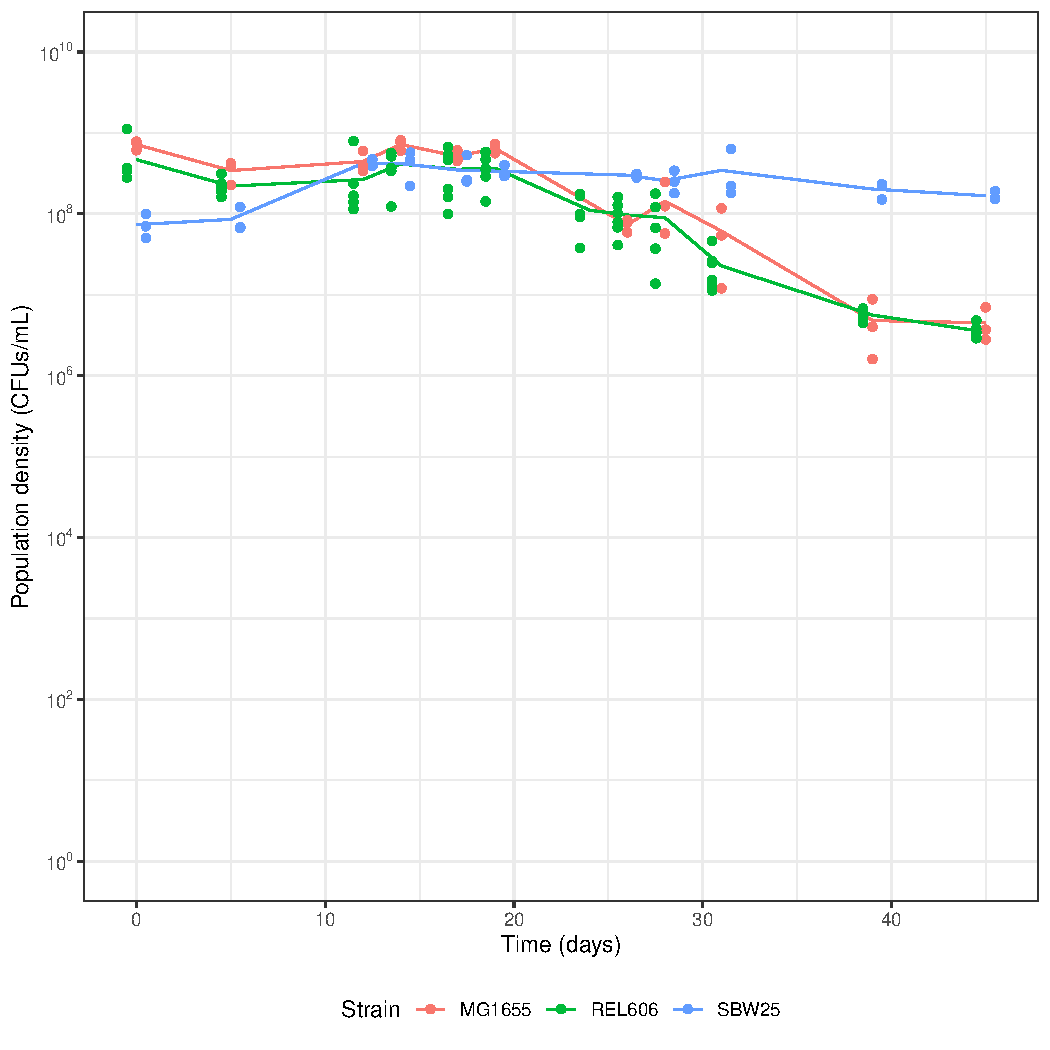
\includegraphics[width=\columnwidth]{mean_plot_LB.pdf}
\captionof{figure}{Semilogarithmic plot of the average population density of SBW25, MG1655, and REL606 in rich medium (LB) at different time points. Dots are single measurements, lines represent the average population density of the different strains.}
\vspace{2ex}

In minimal medium, SBW25 and REL606 maintained a trend similar to that observed in rich medium.
On the contrary, MG1655 showed a markedly different behavior.
\\[2ex]
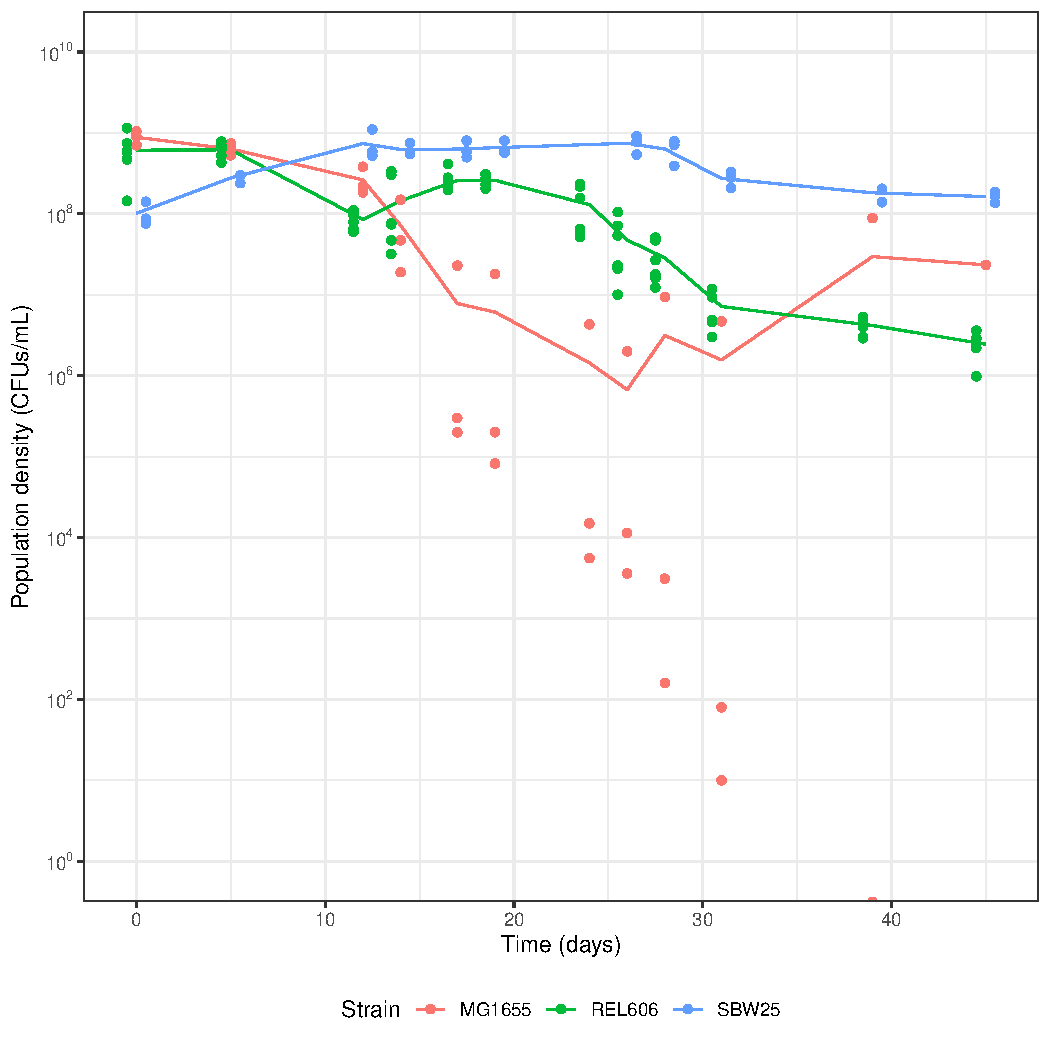
\includegraphics[width=\columnwidth]{mean_plot_M9.pdf}
\captionof{figure}{Semilogarithmic plot of the average population density of SBW25, MG1655 and REL606 in minimal medium (M9) at different time points. Dots are single measurements, lines represent the average population density of the different strains.}
\vspace{2ex}

Two of the MG1655 replicates in M9 began a steep decline in population density after day 12, which ended at day 39 with the complete disappearance of regeneration capacity (no colonies developed after inoculation of 100 $\mu$L of undiluted culture in M9-agar plates).
This was confirmed by inoculating 200 $\mu$L of the two cultures in 2 mL of liquid M9 medium.
After overnight incubation, the optical density of the medium did not show any increase.
The remaining MG1655 replicate instead showed an initial decline, followed by an increase in population density after day 17.
\\[2ex]
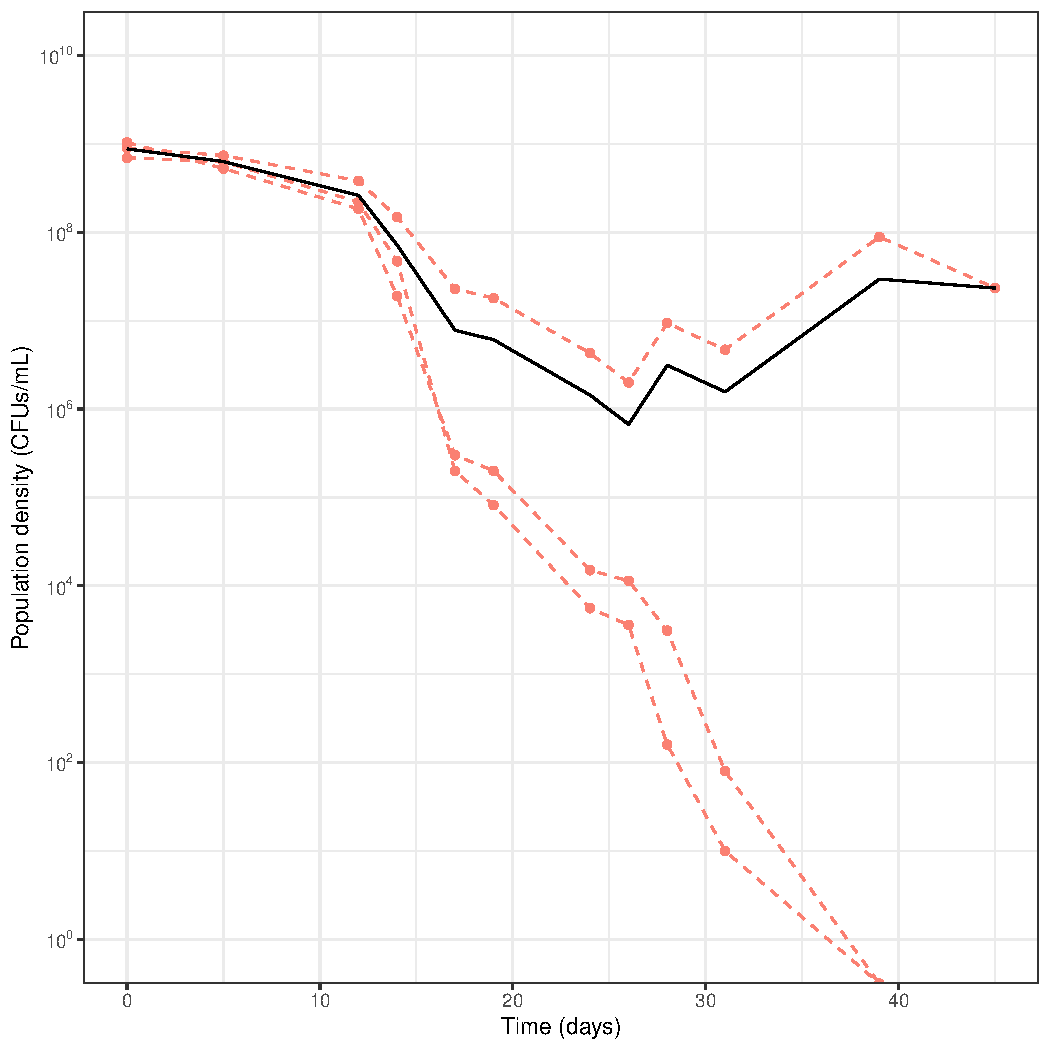
\includegraphics[width=\columnwidth]{MG1655_M9_plot.pdf}
\captionof{figure}{Semilogarithmic plot of the average population density of MG1655 in minimal medium (M9) at different time points. Dots are single measurements, the dotted lines connect measurements of the same replicate. The solid line is the average across replicates.}

\subsection*{Evolution of phenotypic diversity in SBW25}
During the course of the experiment, SBW25 developed different colony morphologies.
The evolution of phenotypic diversity was almost exclusive of the samples in rich medium.
Only 2 wrinkly spreader colonies were observed in minimal medium, one at day 39 (139 colonies in total) and one at day 45 (167 colonies in total), in the same replicate.
Wrinkly spreaders developped in all the LB samples, however one of the replicates showed exclusively a larger variety of wrinkly spreaders (see image \ref{bWS_col}), while another showed a wast majority of a smaller variety of wrinkly spreaders (see image \ref{sWS_col}).
\\[2ex]
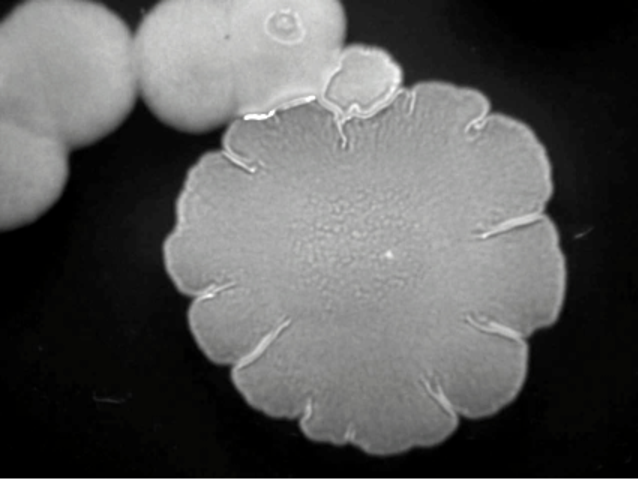
\includegraphics[width=\columnwidth]{bWS_col.pdf}
\label{bWS_col}
\captionof{figure}{SBW25 in LB-agar plate. Large variety of wrinkly spreader colony surrounded by smooth morph colonies.}
\vspace{2ex}

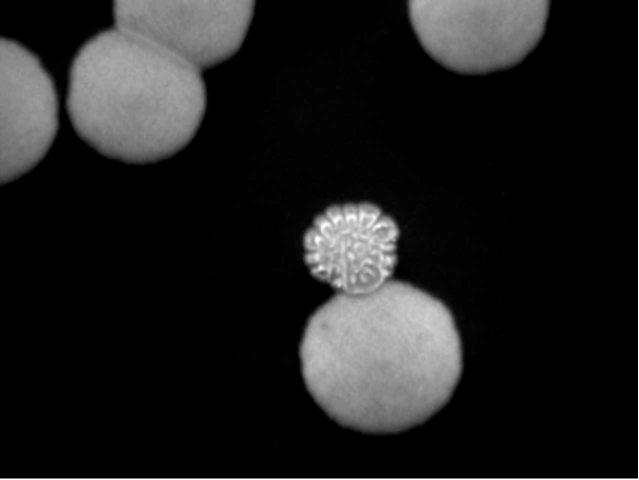
\includegraphics[width=\columnwidth]{sWS_col.pdf}
\label{sWS_col}
\captionof{figure}{SBW25 in LB-agar plate. Small variety of wrinkly spreader colony surrounded by smooth morph colonies.}
\vspace{2ex}
In the third replicate only a small number of wrinkly spreaders appeared.
Diversity increased in all samples in the first phase of the experiment, peaked around day 20 and then started to decline. 
\\[2ex]
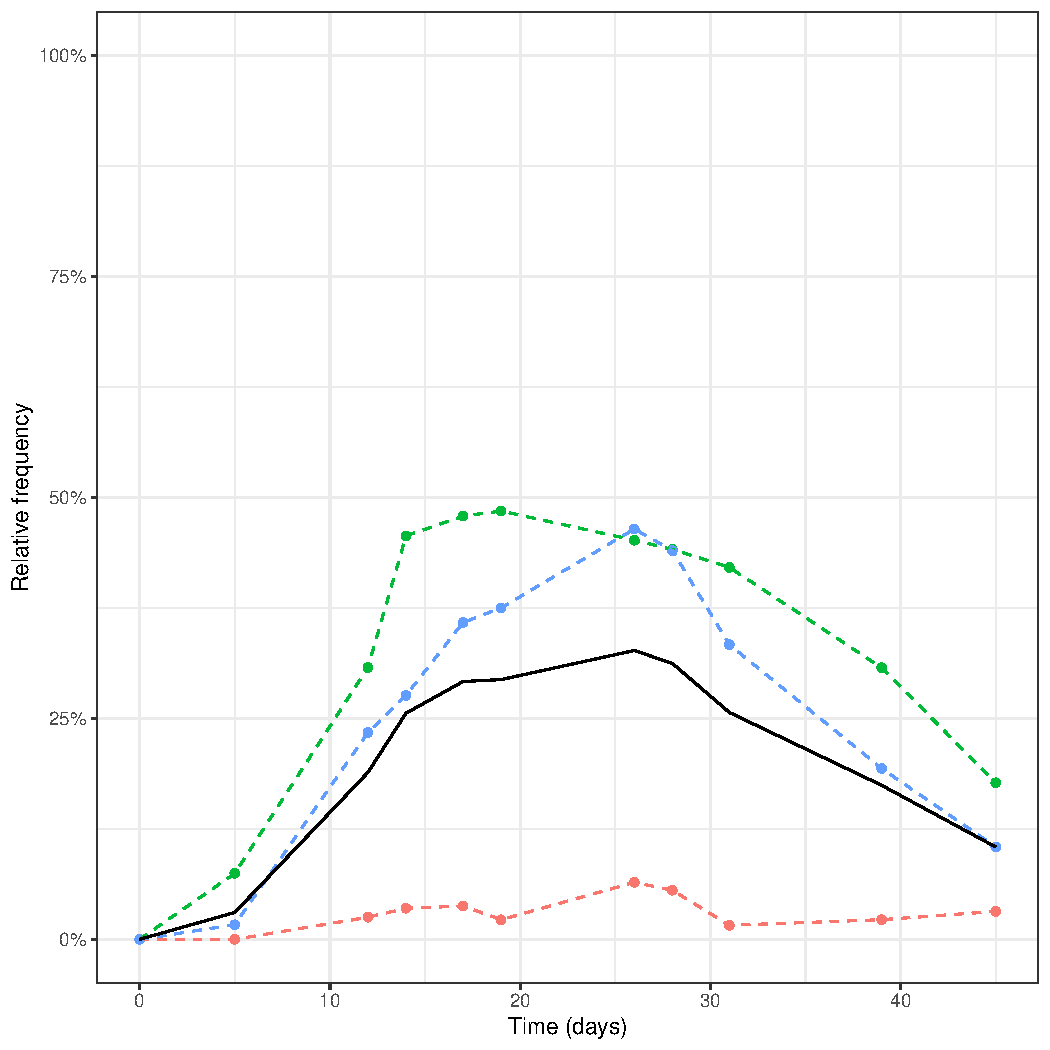
\includegraphics[width=\columnwidth]{WS_plot.pdf}
\captionof{figure}{Plot of the relative abundance of wrinkly spreaders in the three SBW25 samples in rich medium. The colored, dotted lines represent the three replicates. The solid line represents the average.}
\vspace{2ex}

Fuzzy spreaders (see image \ref{FS_col}) started to appear towards the end of the experiment in two of the SBW25 samples in LB.
\\[2ex]
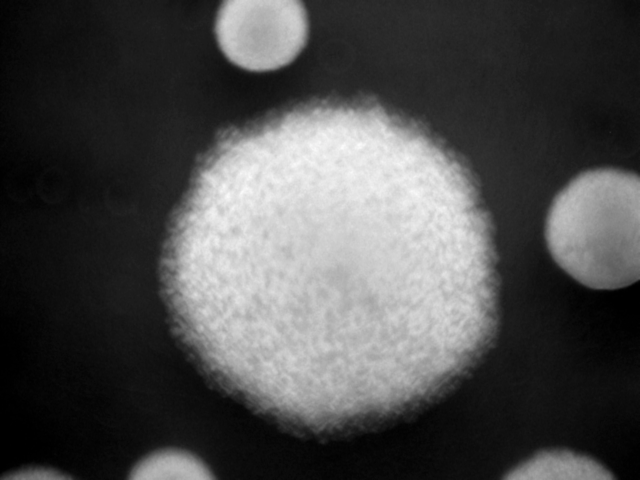
\includegraphics[width=\columnwidth]{FS_col.pdf}
\label{FS_col}
\captionof{figure}{SBW25 in LB-agar plate. Fuzzy spreader colony surrounded by smooth morph colonies.}
\vspace{2ex}
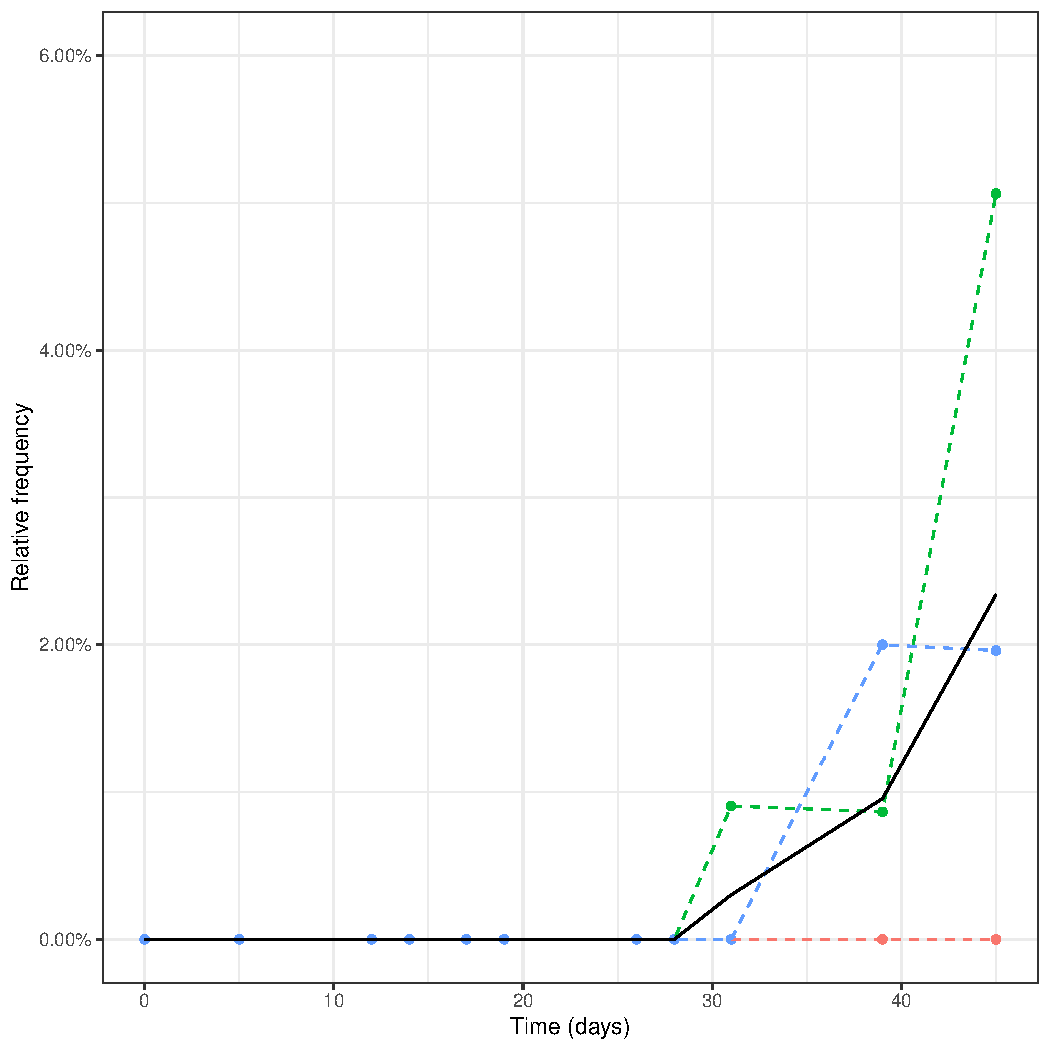
\includegraphics[width=\columnwidth]{FS_plot.pdf}
\captionof{figure}{Plot of the relative abundance of fuzzy spreaders in the three SBW25 samples in rich medium. The colored, dotted lines represent the three replicates. The solid line represents the average. Note that, in order to better visualize the data, the x-axis does not show the entire 0-100\% range (0-6\% is shown).}
\vspace{2ex}

\subsection*{Appearance of small colonies in \textit{E. coli}}
In both \textit{E. coli} strains (MG1655 and REL606) the appearance of small colonies was observed, mainly in rich medium.
They appeared in REL606 in LB at day 12 and remained abundant since then.
In MG1655 they appeared later and increased in frequency with a slower pace, but reached a comparable frequency towards the end of the experiment.
In minimal medium, small colonies were not initially observed but started to appear in REL606 on day 39.
No variation in colony size was observed for SBW25.
\\[2ex]
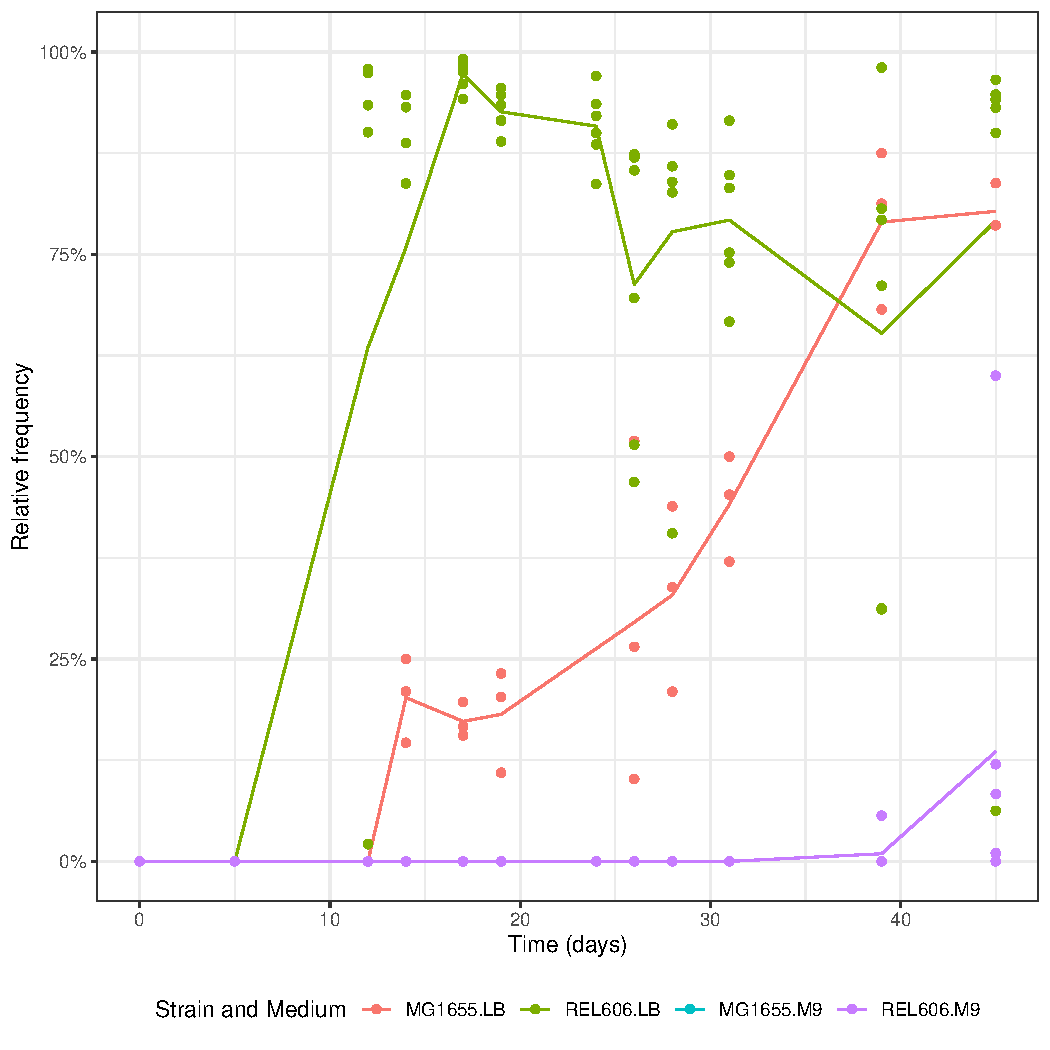
\includegraphics[width=\columnwidth]{small_plot_report.pdf}
\captionof{figure}{Plot of the average relative number of small colonies in MG1655 and REL606, in rich (LB) and minimal (M9) medium. The lines represent the average across replicates, the dots are single measurements.}
\vspace{2ex}

\section*{Discussion}
The observed survival of the three bacterial strains over 45 days is not particularly surprising since it has been reported that \textit{E. coli} can survive in similar conditions for years \citep{Finkel1999}.

The disappearance in regeneration capacity observed in two MG1655 replicates grown in minimal medium was unexpected.
The different behavior of the three replicates could be explained by the occurrence of a rare mutation in the surviving sample.
In order to test this hypothesis, it could be interesting to sequence the genome of the surviving strain.
Moreover, repeating the experiment in larger volumes can make rare mutation more probable, thus enhancing consistency across replicates.\\

The evolution of morphological diversity in SBW25 colonies in a non-spatially structured microcosm is interesting because the competitive advantage of wrinkly and fuzzy spreaders is thought to be dependent on the presence of a spatially-structured environment \citep{Rainey1998}.
Their appearance in this setting suggests that wrinkly and fuzzy spreaders could possess some advantageous trait even in a shaken microcosm.
It would be interesting to asses the mechanistic basis of this advantage.\\

The appearance of small colonies in \textit{E. coli} in a variety of stressful conditions has been previously reported \citep{Colwell1946, Santos2016, Tashiro2017}.
It seems reasonable that when subjected to nutrient starvation and deprived of a waste outflow, slow-growing bacterial cells can be selected.
Slow-growing colonies would then translate to smaller colonies when compared to fast-growing ones, at any given time point.
Nonetheless, it would be interesting to asses if the small colony variants that arose in this experiment are hereditable, and to determine the genetic basis of this phenotype.\\

The much lower rate of appearance of variant morphologies (wrinkly spreaders, fuzzy spreaders, small colonies) in minimal medium compared to rich medium is intriguing.
In the case of wrinkly and fuzzy spreaders, a reasonable explanation could be that these phenotypes require more energy to be maintained (for example for the production of the polymer that allows wrinkly spreaders to adhere to each other) and thus they are not advantageous in a more nutrient-limited environment.
In the case of small colonies, there is no obvious explanation.
The slower growth rate in minimal medium (compared to rich medium) could make it more difficult for small, slower-growing variants to emerge.
The reason could be that in minimal medium these variants would grow so slowly that they are not competitive, or not easily detectable by plating with normal incubation times.

\section*{Materials and Methods}

\subsection*{Bacterial strains and start of the experiment}
Three bacterial strains were used: the \textit{E. coli} K-12 strain MG1655 (reference genome: NC\_000913), the \textit{E. coli} B strain REL606 (reference genome: NC\_012967) and the \textit{P. fluorescens} strain SBW25 (reference genome: NC\_012660).
Glycerol stocks of the ancestral strains were streaked on LB-agar and M9-agar plates, so to isolate single colonies.
Three MG1655 colonies, three SBW25 colonies and six REL606 colonies from the LB-agar plates were inoculated in 4 mL of LB liquid medium, in 13 mL tubes with push-down lid.
The same number of colonies was picked from the M9-agar plates and inoculated in M9 liquid medium.
The cultures were incubated overnight at 28$^\circ$C (SBW25) or 37$^\circ$C (MG1655 and REL606) in shaking (200 rpm).

\subsection*{Experimental design}
The long-term cultures were set up in 4 mL of liquid medium (LB or M9), in 13 mL tubes with push-down lid.
These were inoculated using 4 $\mu$L form the respective overnight cultures, marking day 0 of the experiment.
The long-term stationary phase experiment was carried out with 3 MG1655 replicates in LB, 3 MG1655 replicates in M9, 3 SBW25 replicates in LB, 3 SBW25 replicates in M9, 6 REL606 replicates in LB and 6 REL606 replicates in M9.
These samples were maintained at 37$^\circ$C (MG1655 and REL606) or 28$^\circ$C (SBW25) in shaking (200 rpm) for the entire duration of the experiment.
Every 7 days, or more often in some instances (depending on the expected rate of change in population size over time) the samples were stored as glycerol stocks and the population size was monitored.
The volume of the long-term cultures was maintained constant by adding sterile distilled water when needed.

\subsection*{Monitoring of population size}
Periodically, the number population density of the samples was monitored by dilution plating.
Dilution plating was carried out using M9-agar plates for the samples in liquid M9 medium, and LB plates for the samples in liquid LB medium.
Serial dilutions of the cultures were made using Ringer's solution.

\subsection*{Storage of the samples as glycerol stocks}
Every time the population size was monitored by dilution plating, the population state was also preserved as a glycerol stock.
2 $\mu$L were taken from the long-term cultures and used for inoculating 2 mL of LB or M9 liquid medium, in 13 mL tubes with push-down lid.
These tubes were grown overnight at 37$^\circ$C (MG1655 and REL606) or 28$^\circ$C (SBW25) in shaking (200 rpm).
1 mL of the overnight culture was then mixed with 800 $\mu$L of glycerol saline solution and stored at -80$^\circ$C.

\subsection*{Confirmation of strain identity by PCR}
Cross-contamination in the long term-cultures and the identity of single colonies were checked by PCR using strain specific-primers.
These primers were designed so to give an amplification product in one of the three strains, but not in the others.
For SBW25 the primers (FW: 5’-ATACTACGACTCCAGAGCGATGG-3', RV: 5’-GTTCAGCGTCTGCGTGGCTTG-3') amplified a portion of the \textit{pflu3656} gene (Gene ID: 7818868).
For MG1655 the primers (FW: 5’-CTGAATCGGTCATGATGATGGGGACTG-3', RV: 5’-TTCAGGCGGACTTACTATCCCG-3') amplified a portion of the \textit{fliR} gene (Gene ID: 946464).
For REL606 the primers (FW: 5’-CAGTGGATTGTGGTTTGTTGCC-3', RV: 5’-GGCTGGTACTTTTCAGGTCGG-3') amplified a portion of the \textit{hpaA} gene (Gene ID: 8178255).
Primers were used at a 0.8 $\mu$M final concentration.
PCR reactions were carried out with the following program: 94$^\circ$ for 10 minutes, 30 cycles (94$^\circ$ for 30 seconds, 60$^\circ$ for 30 seconds, 72$^\circ$ for 1 minute), 72$^\circ$ for 5 minutes.
The template was obtained by resuspending 1 $\mu$L of liquid culture (or a single colony in case of plates) in 20 $\mu$L of sterile distilled $H_2O$.
0.5 $\mu$L of this suspension were used as PCR template.

\footnotesize
\bibliography{report_mpi_saul}

\end{multicols}

\end{document}

%% NOTES ------------------------------------------------------------------------
% Abstract
% 
% Intro
%
% Results
%     Single MG replicates M9 graph to be put
% Discussion
%
% MM
%
% Ref
%
